

\subsection{Shu-Osher Tube Test}

Shu, C and Osher, S., "Efficient Implementation of Essentially Non-Oscillatory Shock-Capturing 
Schemes, II", J. Computational Physics, 83, 32-78 (1989). The test is Example 8. 

The grid is divided into two parts, with the left containing a uniform postshock flow and the right containing a sinusoidal 
entropy wave.

\subsubsection{Initial Conditions}

Boundary conditions are constant around the X axis and periodic everywhere else.

The physical input parameters to the Shu-Osher test are:
\begin{itemize}
\item \begin{tt}lambda\end{tt} - Defines the entropy wavenumber in waves/box (Shu-Osher: 8)
\item \begin{tt}mach\end{tt} - Defines the strength of the shockwave (Shu-Osher: 3)
\item \begin{tt}waveAmplitude\end{tt} - Defines the amplitude of the entropy wave $d\rho/\rho$ (Shu-Osher: .2)
\end{itemize}

\subsubsection{Analysis}

\begin{figure*}
\begin{center}
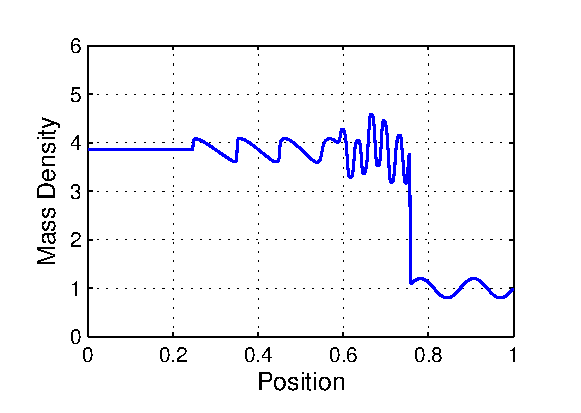
\includegraphics{ShuOsher.eps}
\caption{Shu-Osher Shocktube at t = 0.178}
\end{center}
\end{figure*}

Linearly, the interaction of the shock with the sinusoid modulates the shock strength and generates both entropy and sound
characteristics propagating into the postshock region.

Imogen contains the linear (in infinitesmal entropy wave amplitude) solution and can generate output graphics to compare with.

The interaction of the shock with the entropy waves is a source of immediate nonlinearity. An attempt to solve this to second
order has been made, but this analysis fails to account for other effects of equal order.

Downstream, the sonic characteristics nonlinearly interact with the entropy waves and inevitably steepen up into a train of weak shocks.
In simulations of immensely high resolution (500000 cells), the interaction between the compressed entropy wave and the shock train
seems to be a bottomless fount of 1-dimensional structure.

In the fourier analysis of the shock front's position, peaks corresponding to harmonic distortion, intermodulation 
and self-mixing with up to 6 terms is visible in the log-scale plot. 

